
%% bare_conf.tex
%% V1.3
%% 2007/01/11
%% by Michael Shell
%% See:
%% http://www.michaelshell.org/
%% for current contact information.
%%
%% This is a skeleton file demonstrating the use of IEEEtran.cls
%% (requires IEEEtran.cls version 1.7 or later) with an IEEE conference paper.
%%
%% Support sites:
%% http://www.michaelshell.org/tex/ieeetran/
%% http://www.ctan.org/tex-archive/macros/latex/contrib/IEEEtran/
%% and
%% http://www.ieee.org/

%%*************************************************************************
%% Legal Notice:
%% This code is offered as-is without any warranty either expressed or
%% implied; without even the implied warranty of MERCHANTABILITY or
%% FITNESS FOR A PARTICULAR PURPOSE! 
%% User assumes all risk.
%% In no event shall IEEE or any contributor to this code be liable for
%% any damages or losses, including, but not limited to, incidental,
%% consequential, or any other damages, resulting from the use or misuse
%% of any information contained here.
%%
%% All comments are the opinions of their respective authors and are not
%% necessarily endorsed by the IEEE.
%%
%% This work is distributed under the LaTeX Project Public License (LPPL)
%% ( http://www.latex-project.org/ ) version 1.3, and may be freely used,
%% distributed and modified. A copy of the LPPL, version 1.3, is included
%% in the base LaTeX documentation of all distributions of LaTeX released
%% 2003/12/01 or later.
%% Retain all contribution notices and credits.
%% ** Modified files should be clearly indicated as such, including  **
%% ** renaming them and changing author support contact information. **
%%
%% File list of work: IEEEtran.cls, IEEEtran_HOWTO.pdf, bare_adv.tex,
%%                    bare_conf.tex, bare_jrnl.tex, bare_jrnl_compsoc.tex
%%*************************************************************************

% *** Authors should verify (and, if needed, correct) their LaTeX system  ***
% *** with the testflow diagnostic prior to trusting their LaTeX platform ***
% *** with production work. IEEE's font choices can trigger bugs that do  ***
% *** not appear when using other class files.                            ***
% The testflow support page is at:
% http://www.michaelshell.org/tex/testflow/



% Note that the a4paper option is mainly intended so that authors in
% countries using A4 can easily print to A4 and see how their papers will
% look in print - the typesetting of the document will not typically be
% affected with changes in paper size (but the bottom and side margins will).
% Use the testflow package mentioned above to verify correct handling of
% both paper sizes by the user's LaTeX system.
%
% Also note that the "draftcls" or "draftclsnofoot", not "draft", option
% should be used if it is desired that the figures are to be displayed in
% draft mode.
%
\documentclass[10pt,conference]{IEEEtran}
% Add the compsoc option for Computer Society conferences.
%
% If IEEEtran.cls has not been installed into the LaTeX system files,
% manually specify the path to it like:
% \documentclass[conference]{../sty/IEEEtran}




% Some very useful LaTeX packages include:
% (uncomment the ones you want to load)


% *** MISC UTILITY PACKAGES ***
%
%\usepackage{ifpdf}
% Heiko Oberdiek's ifpdf.sty is very useful if you need conditional
% compilation based on whether the output is pdf or dvi.
% usage:
% \ifpdf
%   % pdf code
% \else
%   % dvi code
% \fi
% The latest version of ifpdf.sty can be obtained from:
% http://www.ctan.org/tex-archive/macros/latex/contrib/oberdiek/
% Also, note that IEEEtran.cls V1.7 and later provides a builtin
% \ifCLASSINFOpdf conditional that works the same way.
% When switching from latex to pdflatex and vice-versa, the compiler may
% have to be run twice to clear warning/error messages.






% *** CITATION PACKAGES ***
%
%\usepackage{cite}
% cite.sty was written by Donald Arseneau
% V1.6 and later of IEEEtran pre-defines the format of the cite.sty package
% \cite{} output to follow that of IEEE. Loading the cite package will
% result in citation numbers being automatically sorted and properly
% "compressed/ranged". e.g., [1], [9], [2], [7], [5], [6] without using
% cite.sty will become [1], [2], [5]--[7], [9] using cite.sty. cite.sty's
% \cite will automatically add leading space, if needed. Use cite.sty's
% noadjust option (cite.sty V3.8 and later) if you want to turn this off.
% cite.sty is already installed on most LaTeX systems. Be sure and use
% version 4.0 (2003-05-27) and later if using hyperref.sty. cite.sty does
% not currently provide for hyperlinked citations.
% The latest version can be obtained at:
% http://www.ctan.org/tex-archive/macros/latex/contrib/cite/
% The documentation is contained in the cite.sty file itself.






% *** GRAPHICS RELATED PACKAGES ***
%
\ifCLASSINFOpdf
  % \usepackage[pdftex]{graphicx}
  % declare the path(s) where your graphic files are
  % \graphicspath{{../pdf/}{../jpeg/}}
  % and their extensions so you won't have to specify these with
  % every instance of \includegraphics
  % \DeclareGraphicsExtensions{.pdf,.jpeg,.png}
\else
  % or other class option (dvipsone, dvipdf, if not using dvips). graphicx
  % will default to the driver specified in the system graphics.cfg if no
  % driver is specified.
  % \usepackage[dvips]{graphicx}
  % declare the path(s) where your graphic files are
  % \graphicspath{{../eps/}}
  % and their extensions so you won't have to specify these with
  % every instance of \includegraphics
  % \DeclareGraphicsExtensions{.eps}
\fi
% graphicx was written by David Carlisle and Sebastian Rahtz. It is
% required if you want graphics, photos, etc. graphicx.sty is already
% installed on most LaTeX systems. The latest version and documentation can
% be obtained at: 
% http://www.ctan.org/tex-archive/macros/latex/required/graphics/
% Another good source of documentation is "Using Imported Graphics in
% LaTeX2e" by Keith Reckdahl which can be found as epslatex.ps or
% epslatex.pdf at: http://www.ctan.org/tex-archive/info/
%
% latex, and pdflatex in dvi mode, support graphics in encapsulated
% postscript (.eps) format. pdflatex in pdf mode supports graphics
% in .pdf, .jpeg, .png and .mps (metapost) formats. Users should ensure
% that all non-photo figures use a vector format (.eps, .pdf, .mps) and
% not a bitmapped formats (.jpeg, .png). IEEE frowns on bitmapped formats
% which can result in "jaggedy"/blurry rendering of lines and letters as
% well as large increases in file sizes.
%
% You can find documentation about the pdfTeX application at:
% http://www.tug.org/applications/pdftex





% *** MATH PACKAGES ***
%
\usepackage[cmex10]{amsmath}
\usepackage{amsthm}
\usepackage[x11names, rgb]{xcolor}
\usepackage[utf8]{inputenc}
\usepackage{tikz}
\usetikzlibrary{snakes,arrows,shapes}
% A popular package from the American Mathematical Society that provides
% many useful and powerful commands for dealing with mathematics. If using
% it, be sure to load this package with the cmex10 option to ensure that
% only type 1 fonts will utilized at all point sizes. Without this option,
% it is possible that some math symbols, particularly those within
% footnotes, will be rendered in bitmap form which will result in a
% document that can not be IEEE Xplore compliant!
%
% Also, note that the amsmath package sets \interdisplaylinepenalty to 10000
% thus preventing page breaks from occurring within multiline equations. Use:
%\interdisplaylinepenalty=2500
% after loading amsmath to restore such page breaks as IEEEtran.cls normally
% does. amsmath.sty is already installed on most LaTeX systems. The latest
% version and documentation can be obtained at:
% http://www.ctan.org/tex-archive/macros/latex/required/amslatex/math/





% *** SPECIALIZED LIST PACKAGES ***
%
%\usepackage{algorithmic}
% algorithmic.sty was written by Peter Williams and Rogerio Brito.
% This package provides an algorithmic environment fo describing algorithms.
% You can use the algorithmic environment in-text or within a figure
% environment to provide for a floating algorithm. Do NOT use the algorithm
% floating environment provided by algorithm.sty (by the same authors) or
% algorithm2e.sty (by Christophe Fiorio) as IEEE does not use dedicated
% algorithm float types and packages that provide these will not provide
% correct IEEE style captions. The latest version and documentation of
% algorithmic.sty can be obtained at:
% http://www.ctan.org/tex-archive/macros/latex/contrib/algorithms/
% There is also a support site at:
% http://algorithms.berlios.de/index.html
% Also of interest may be the (relatively newer and more customizable)
% algorithmicx.sty package by Szasz Janos:
% http://www.ctan.org/tex-archive/macros/latex/contrib/algorithmicx/




% *** ALIGNMENT PACKAGES ***
%
%\usepackage{array}
% Frank Mittelbach's and David Carlisle's array.sty patches and improves
% the standard LaTeX2e array and tabular environments to provide better
% appearance and additional user controls. As the default LaTeX2e table
% generation code is lacking to the point of almost being broken with
% respect to the quality of the end results, all users are strongly
% advised to use an enhanced (at the very least that provided by array.sty)
% set of table tools. array.sty is already installed on most systems. The
% latest version and documentation can be obtained at:
% http://www.ctan.org/tex-archive/macros/latex/required/tools/


%\usepackage{mdwmath}
%\usepackage{mdwtab}
% Also highly recommended is Mark Wooding's extremely powerful MDW tools,
% especially mdwmath.sty and mdwtab.sty which are used to format equations
% and tables, respectively. The MDWtools set is already installed on most
% LaTeX systems. The lastest version and documentation is available at:
% http://www.ctan.org/tex-archive/macros/latex/contrib/mdwtools/


% IEEEtran contains the IEEEeqnarray family of commands that can be used to
% generate multiline equations as well as matrices, tables, etc., of high
% quality.


%\usepackage{eqparbox}
% Also of notable interest is Scott Pakin's eqparbox package for creating
% (automatically sized) equal width boxes - aka "natural width parboxes".
% Available at:
% http://www.ctan.org/tex-archive/macros/latex/contrib/eqparbox/





% *** SUBFIGURE PACKAGES ***
%\usepackage[tight,footnotesize]{subfigure}
% subfigure.sty was written by Steven Douglas Cochran. This package makes it
% easy to put subfigures in your figures. e.g., "Figure 1a and 1b". For IEEE
% work, it is a good idea to load it with the tight package option to reduce
% the amount of white space around the subfigures. subfigure.sty is already
% installed on most LaTeX systems. The latest version and documentation can
% be obtained at:
% http://www.ctan.org/tex-archive/obsolete/macros/latex/contrib/subfigure/
% subfigure.sty has been superceeded by subfig.sty.



%\usepackage[caption=false]{caption}
%\usepackage[font=footnotesize]{subfig}
% subfig.sty, also written by Steven Douglas Cochran, is the modern
% replacement for subfigure.sty. However, subfig.sty requires and
% automatically loads Axel Sommerfeldt's caption.sty which will override
% IEEEtran.cls handling of captions and this will result in nonIEEE style
% figure/table captions. To prevent this problem, be sure and preload
% caption.sty with its "caption=false" package option. This is will preserve
% IEEEtran.cls handing of captions. Version 1.3 (2005/06/28) and later 
% (recommended due to many improvements over 1.2) of subfig.sty supports
% the caption=false option directly:
%\usepackage[caption=false,font=footnotesize]{subfig}
%
% The latest version and documentation can be obtained at:
% http://www.ctan.org/tex-archive/macros/latex/contrib/subfig/
% The latest version and documentation of caption.sty can be obtained at:
% http://www.ctan.org/tex-archive/macros/latex/contrib/caption/




% *** FLOAT PACKAGES ***
%
%\usepackage{fixltx2e}
% fixltx2e, the successor to the earlier fix2col.sty, was written by
% Frank Mittelbach and David Carlisle. This package corrects a few problems
% in the LaTeX2e kernel, the most notable of which is that in current
% LaTeX2e releases, the ordering of single and double column floats is not
% guaranteed to be preserved. Thus, an unpatched LaTeX2e can allow a
% single column figure to be placed prior to an earlier double column
% figure. The latest version and documentation can be found at:
% http://www.ctan.org/tex-archive/macros/latex/base/



%\usepackage{stfloats}
% stfloats.sty was written by Sigitas Tolusis. This package gives LaTeX2e
% the ability to do double column floats at the bottom of the page as well
% as the top. (e.g., "\begin{figure*}[!b]" is not normally possible in
% LaTeX2e). It also provides a command:
%\fnbelowfloat
% to enable the placement of footnotes below bottom floats (the standard
% LaTeX2e kernel puts them above bottom floats). This is an invasive package
% which rewrites many portions of the LaTeX2e float routines. It may not work
% with other packages that modify the LaTeX2e float routines. The latest
% version and documentation can be obtained at:
% http://www.ctan.org/tex-archive/macros/latex/contrib/sttools/
% Documentation is contained in the stfloats.sty comments as well as in the
% presfull.pdf file. Do not use the stfloats baselinefloat ability as IEEE
% does not allow \baselineskip to stretch. Authors submitting work to the
% IEEE should note that IEEE rarely uses double column equations and
% that authors should try to avoid such use. Do not be tempted to use the
% cuted.sty or midfloat.sty packages (also by Sigitas Tolusis) as IEEE does
% not format its papers in such ways.





% *** PDF, URL AND HYPERLINK PACKAGES ***
%
%\usepackage{url}
% url.sty was written by Donald Arseneau. It provides better support for
% handling and breaking URLs. url.sty is already installed on most LaTeX
% systems. The latest version can be obtained at:
% http://www.ctan.org/tex-archive/macros/latex/contrib/misc/
% Read the url.sty source comments for usage information. Basically,
% \url{my_url_here}.


\usepackage{amsmath}
\usepackage{amsfonts}
\usepackage{amssymb}
\usepackage{amsthm}
%\usepackage{bbold}
\usepackage{xspace}
\usepackage{array}
\usepackage[figuresleft]{rotating}
\usepackage{multirow}
\usepackage{color}

\newcolumntype{R}{>{$}r<{$}}
\newcolumntype{L}{>{$}l<{$}}
\newcolumntype{C}{>{$}c<{$}}

\newcommand{\mtt}[1]{\ensuremath{\mathit{#1}}}
\newcommand{\anywhere}[1]{\ensuremath{\mbox{#1}}}
\newcommand{\kw}[1]{\anywhere{\sffamily{\bfseries\small {#1}}}}
\newcommand{\red}[1]{{\color{red}{#1}}}
\newcommand{\note}[1]{\red{\textbf{[#1]}}}
\newcommand{\nvsp}{\vspace{-.1in}}
\newcommand{\ignore}[1]{}

\newcommand{\alt}{\ \mid\ }
\newcommand{\lalt}{\ \ \ \alt}


\newcommand{\N}{\mathbb{N}}
\newcommand{\B}{\mathbb{B}}
\newcommand{\I}{\mathcal{I}}
\newcommand{\Oo}{\mathcal{O}}
\newcommand{\Set}{\mathcal{P}}

\newcommand{\step}{\ensuremath{\mathcal{F}}\xspace}

\newcommand{\To}{\Rightarrow}

\newcommand{\Prog}{\ensuremath{\mtt{Prog}\xspace}}
\newcommand{\BitVector}{\ensuremath{\mtt{BitVector}\xspace}}
\newcommand{\MemUnit}{\ensuremath{\mtt{MemUnit}\xspace}}
\newcommand{\RegVals}{\ensuremath{\mtt{RegVals}\xspace}}
\newcommand{\MemVals}{\ensuremath{\mtt{MemVals}\xspace}}
\newcommand{\EdgeWidths}{\ensuremath{\mtt{EdgeWidths}\xspace}}
\newcommand{\EdgeVals}{\ensuremath{\mtt{EdgeVals}\xspace}}
\newcommand{\MemLabel}{\ensuremath{\mtt{MemLabel}\xspace}}
\newcommand{\EdgeLabel}{\ensuremath{\mtt{EdgeLabel}\xspace}}
\newcommand{\RegLabel}{\ensuremath{\mtt{RegLabel}\xspace}}
\newcommand{\RegMap}{\ensuremath{\mtt{RegMap}\xspace}}
\newcommand{\MemMap}{\ensuremath{\mtt{MemMap}\xspace}}
\newcommand{\Bool}{\ensuremath{\B = \{0, 1 \} } }
\newcommand{\Bits}{\ensuremath{\mtt{Bits}}\xspace}
\newcommand{\String}{\ensuremath{\mtt{String}\xspace}}
\newcommand{\Data}{\ensuremath{\mtt{Data}\xspace}}
\newcommand{\Node}{\ensuremath{\mtt{Node}\xspace}}
\newcommand{\Mux}{\ensuremath{\kw{mux}}\xspace}
\newcommand{\Slice}{\ensuremath{\mtt{Slice}\xspace}}
\newcommand{\Memory}{\ensuremath{\mtt{Memory}\xspace}}
\newcommand{\Register}{\ensuremath{\mtt{Register}\xspace}}
\newcommand{\Input}{\ensuremath{\kw{in}\xspace}}
\newcommand{\Output}{\ensuremath{\kw{out}\xspace}}
\newcommand{\Literal}{\ensuremath{\kw{lit}\xspace}}
\newcommand{\Label}{\ensuremath{\mtt{Label}\xspace}}
\newcommand{\Edge}{\ensuremath{\mtt{Edge}\xspace}}
\newcommand{\Graph}{\ensuremath{\mtt{Graph}\xspace}}
\newcommand{\NodeStore}{\ensuremath{\mtt{NStore}\xspace}}
\newcommand{\MemStore}{\ensuremath{\mtt{MStore}\xspace}}
\newcommand{\State}{\ensuremath{\mtt{State}\xspace}}
\newcommand{\CMemRead}{\ensuremath{\mtt{CMemRead}} \xspace}
\newcommand{\CMemWrite}{\ensuremath{\mtt{CMemWrite}} \xspace}
\newcommand{\SMemRead}{\ensuremath{\mtt{SMemRead}} \xspace}
\newcommand{\SMemWrite}{\ensuremath{\mtt{SMemWrite}} \xspace}
\newcommand{\MemRead}{\ensuremath{\kw{memR}} \xspace}
\newcommand{\MemWrite}{\ensuremath{\kw{memW}} \xspace}
\newcommand{\UpdateReg}{\ensuremath{\mtt{UpdateReg}} \xspace}
\newcommand{\Reg}{\ensuremath{\kw{reg}} \xspace}



\newcommand{\BinOp}{\ensuremath{\mtt{BinOp} \xspace}}
\newcommand{\UnOp}{\ensuremath{\mtt{UnOp} \xspace}}


\newcommand{\xor}{\ensuremath{\veebar}}
\newcommand{\bop}{\ensuremath{\oplus}}
\newcommand{\uop}{\ensuremath{\odot}}
\newcommand{\rsh}{>\!\!>}
\newcommand{\lsh}{<\!\!<}
\newcommand{\cat}{+\!\!+\xspace}

\newcommand{\dc}{\ensuremath{\underline{\;\;}}\xspace}




% *** Do not adjust lengths that control margins, column widths, etc. ***
% *** Do not use packages that alter fonts (such as pslatex).         ***
% There should be no need to do such things with IEEEtran.cls V1.6 and later.
% (Unless specifically asked to do so by the journal or conference you plan
% to submit to, of course. )


% correct bad hyphenation here
\hyphenation{op-tical net-works semi-conduc-tor}


\begin{document}
%
% paper title
% can use linebreaks \\ within to get better formatting as desired
\title{Critic: Designing a Sound Static Analyzer for Chisel}

% author names and affiliations
% use a multiple column layout for up to three different
% affiliations
\author{\IEEEauthorblockN{Ethan A. Kuefner, Timothy Sherwood, Ben Hardekopf}
\IEEEauthorblockA{University of California, Santa Barbara\\
\{eakuefner, sherwood, benh\}@cs.ucsb.edu
}
\and
\IEEEauthorblockN{John Sarracino}
\IEEEauthorblockA{Harvey Mudd College\\
jsarracino@g.hmc.edu}}

% conference papers do not typically use \thanks and this command
% is locked out in conference mode. If really needed, such as for
% the acknowledgment of grants, issue a \IEEEoverridecommandlockouts
% after \documentclass

% for over three affiliations, or if they all won't fit within the width
% of the page, use this alternative format:
% 
%\author{\IEEEauthorblockN{Michael Shell\IEEEauthorrefmark{1},
%Homer Simpson\IEEEauthorrefmark{2},
%James Kirk\IEEEauthorrefmark{3}, 
%Montgomery Scott\IEEEauthorrefmark{3} and
%Eldon Tyrell\IEEEauthorrefmark{4}}
%\IEEEauthorblockA{\IEEEauthorrefmark{1}School of Electrical and Computer Engineering\\
%Georgia Institute of Technology,
%Atlanta, Georgia 30332--0250\\ Email: see http://www.michaelshell.org/contact.html}
%\IEEEauthorblockA{\IEEEauthorrefmark{2}Twentieth Century Fox, Springfield, USA\\
%Email: homer@thesimpsons.com}
%\IEEEauthorblockA{\IEEEauthorrefmark{3}Starfleet Academy, San Francisco, California 96678-2391\\
%Telephone: (800) 555--1212, Fax: (888) 555--1212}
%\IEEEauthorblockA{\IEEEauthorrefmark{4}Tyrell Inc., 123 Replicant Street, Los Angeles, California 90210--4321}}




% use for special paper notices
%\IEEEspecialpapernotice{(Invited Paper)}




% make the title area
\maketitle


%\begin{abstract}
%\boldmath
%The abstract goes here.
%\end{abstract}
% IEEEtran.cls defaults to using nonbold math in the Abstract.
% This preserves the distinction between vectors and scalars. However,
% if the conference you are submitting to favors bold math in the abstract,
% then you can use LaTeX's standard command \boldmath at the very start
% of the abstract to achieve this. Many IEEE journals/conferences frown on
% math in the abstract anyway.

% no keywords




% For peer review papers, you can put extra information on the cover
% page as needed:
% \ifCLASSOPTIONpeerreview
% \begin{center} \bfseries EDICS Category: 3-BBND \end{center}
% \fi
%
% For peerreview papers, this IEEEtran command inserts a page break and
% creates the second title. It will be ignored for other modes.
\IEEEpeerreviewmaketitle



\section{Introduction}
% no \IEEEPARstart
For hardware designers, testing is commonplace as a way to ensure
that hardware designs meet their specifications. However, in
high assurance settings such as flight systems, medicine, and
defense, strong guarantees on the behavior of a system may be
required. To achieve such guarantees using testing can be tedious
for sufficiently large designs, since achieving suitable test
coverage can require a potentially exponential number of test inputs.
Formal static analysis provides an alternative to testing in which
mathematical models are reasoned about in order to provide provable
guarantees about the operation of a system. Additionally, we can
design analyses to be \emph{sound}, which means that they will only
return answers which are guaranteed to be true. Thus, a static analysis-based 
approach to ensuring conformance of designs can
remove overhead associated with exhaustive testing as well as potentially provide
stronger guarantees than non-exhaustive testing.

While static analysis seems attractive, it is also difficult;
in fact, Rice's theorem states that any non-trivial property of
programs is undecidable. Many approaches exist to deal with this problem,
but in particular, we appeal to the framework of abstract interpretation~\cite{cc77},
which was originally designed as a technique to perform sound analyses
of programs. In abstract interpretation, a formal concrete semantics for a
programming language is given a mathematical correspondance to an abstract
semantics that soundly approximates the behavior of programs.
Abstract interpretation is well-known in the programming
languages community and has even been used commercially in tools like
{\sc Astr\'ee}, which has successfully verified C code for a variety
of avionics software.

Abstract interpretation can be applied to a hardware design setting through
the observation that hardware description languages are essentially a particular
class of
domain-specific languages (DSLs), that is, programming languages designed to target
a specific application. Chisel~\cite{asanovic12} is a new environment for
designing and testing hardware that has been designed as an embedded DSL on top
of the Scala programming language. For hardware designers, it provides
advantages over existing HDLs by bringing advanced features of Scala, such
as higher-order functions and object oriented programming, to the hardware
design landscape. As well, it presents a good opportunity for analysis designers,
since Chisel has been explicitly designed from the ground up for synthesis, 
unlike either VHDL or Verilog. This reins in the size of the language and 
and allows us to more easily reason about the language and its compilation process
as a whole.

This work is the latest in a series of collaborations between the Programming Languages
Lab and the ArchLab towards applying techniques in programming languages to provably
correct hardware design. In this work, we describe the architecture of Critic, an abstract
interpreter we have been designing for Chisel, and our plans for applying it to proving
particular invariants of hardware designs.

% An example of a floating figure using the graphicx package.
% Note that \label must occur AFTER (or within) \caption.
% For figures, \caption should occur after the \includegraphics.
% Note that IEEEtran v1.7 and later has special internal code that
% is designed to preserve the operation of \label within \caption
% even when the captionsoff option is in effect. However, because
% of issues like this, it may be the safest practice to put all your
% \label just after \caption rather than within \caption{}.
%
% Reminder: the "draftcls" or "draftclsnofoot", not "draft", class
% option should be used if it is desired that the figures are to be
% displayed while in draft mode.
%
%\begin{figure}[!t]
%\centering
%\includegraphics[width=2.5in]{myfigure}
% where an .eps filename suffix will be assumed under latex, 
% and a .pdf suffix will be assumed for pdflatex; or what has been declared
% via \DeclareGraphicsExtensions.
%\caption{Simulation Results}
%\label{fig_sim}
%\end{figure}

% Note that IEEE typically puts floats only at the top, even when this
% results in a large percentage of a column being occupied by floats.


% An example of a double column floating figure using two subfigures.
% (The subfig.sty package must be loaded for this to work.)
% The subfigure \label commands are set within each subfloat command, the
% \label for the overall figure must come after \caption.
% \hfil must be used as a separator to get equal spacing.
% The subfigure.sty package works much the same way, except \subfigure is
% used instead of \subfloat.
%
%\begin{figure*}[!t]
%\centerline{\subfloat[Case I]\includegraphics[width=2.5in]{subfigcase1}%
%\label{fig_first_case}}
%\hfil
%\subfloat[Case II]{\includegraphics[width=2.5in]{subfigcase2}%
%\label{fig_second_case}}}
%\caption{Simulation results}
%\label{fig_sim}
%\end{figure*}
%
% Note that often IEEE papers with subfigures do not employ subfigure
% captions (using the optional argument to \subfloat), but instead will
% reference/describe all of them (a), (b), etc., within the main caption.


% An example of a floating table. Note that, for IEEE style tables, the 
% \caption command should come BEFORE the table. Table text will default to
% \footnotesize as IEEE normally uses this smaller font for tables.
% The \label must come after \caption as always.
%
%\begin{table}[!t]
%% increase table row spacing, adjust to taste
%\renewcommand{\arraystretch}{1.3}
% if using array.sty, it might be a good idea to tweak the value of
% \extrarowheight as needed to properly center the text within the cells
%\caption{An Example of a Table}
%\label{table_example}
%\centering
%% Some packages, such as MDW tools, offer better commands for making tables
%% than the plain LaTeX2e tabular which is used here.
%\begin{tabular}{|c||c|}
%\hline
%One & Two\\
%\hline
%Three & Four\\
%\hline
%\end{tabular}
%\end{table}


% Note that IEEE does not put floats in the very first column - or typically
% anywhere on the first page for that matter. Also, in-text middle ("here")
% positioning is not used. Most IEEE journals/conferences use top floats
% exclusively. Note that, LaTeX2e, unlike IEEE journals/conferences, places
% footnotes above bottom floats. This can be corrected via the \fnbelowfloat
% command of the stfloats package.

\newtheorem{definition}{Definition}

\section{Design}

In this section we outline first the process of extracting a hardware description
amenable to analysis from Chisel, and second, the method we use to perform analysis
on it.

\subsection{Chisel}
Chisel itself is merely a set of data structures which hardware designers
instantiate in a particular way to build components. These data structures
together represent a directed acyclic graph (DAG) of nodes such as binary operations,
multiplexers, and
memory reads and writes. Chisel allows extraction
of C++ or Verilog from this DAG, for use in simulation or synthesis. 
When a designer ``programs'' in Chisel, she is actually programming in Scala.
Figure~\cite{fig:overview} gives an overview of the Chisel/Critic workflow.

\begin{figure}
\begin{center}
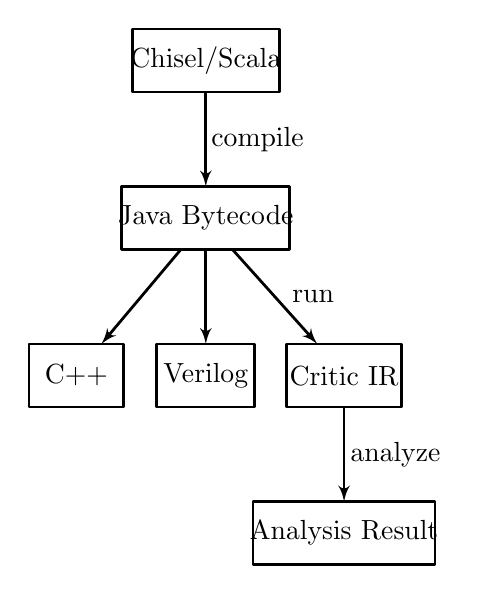
\begin{tikzpicture}[>=latex',line join=bevel,scale=0.63,]
  \pgfsetlinewidth{1bp}
%%
\pgfsetcolor{black}
  % Edge: Java Bytecode -> C++
  \draw [->] (86.38bp,179.61bp) .. controls (75.363bp,166.51bp) and (60.105bp,148.37bp)  .. (41.338bp,126.05bp);
  % Edge: Chisel/Scala -> Java Bytecode
  \draw [->] (101bp,269.61bp) .. controls (101bp,257.24bp) and (101bp,240.37bp)  .. (101bp,216.05bp);
  \definecolor{strokecol}{rgb}{0.0,0.0,0.0};
  \pgfsetstrokecolor{strokecol}
  \draw (130.55bp,243bp) node {compile};
  % Edge: Java Bytecode -> Verilog
  \draw [->] (101bp,179.61bp) .. controls (101bp,167.24bp) and (101bp,150.37bp)  .. (101bp,126.05bp);
  % Edge: Critic IR -> Analysis Result
  \draw [->] (180bp,89.614bp) .. controls (180bp,77.24bp) and (180bp,60.369bp)  .. (180bp,36.05bp);
  \draw (209.37bp,63bp) node {analyze};
  % Edge: Java Bytecode -> Critic IR
  \draw [->] (116.61bp,179.61bp) .. controls (128.37bp,166.51bp) and (144.66bp,148.37bp)  .. (164.69bp,126.05bp);
  \draw (162.33bp,153bp) node {run};
  % Node: Critic IR
\begin{scope}
  \definecolor{strokecol}{rgb}{0.0,0.0,0.0};
  \pgfsetstrokecolor{strokecol}
  \draw (213bp,126bp) -- (147bp,126bp) -- (147bp,90bp) -- (213bp,90bp) -- cycle;
  \draw (180bp,108bp) node {Critic IR};
\end{scope}
  % Node: C++
\begin{scope}
  \definecolor{strokecol}{rgb}{0.0,0.0,0.0};
  \pgfsetstrokecolor{strokecol}
  \draw (54bp,126bp) -- (0bp,126bp) -- (0bp,90bp) -- (54bp,90bp) -- cycle;
  \draw (27bp,108bp) node {C++};
\end{scope}
  % Node: Java Bytecode
\begin{scope}
  \definecolor{strokecol}{rgb}{0.0,0.0,0.0};
  \pgfsetstrokecolor{strokecol}
  \draw (149bp,216bp) -- (53bp,216bp) -- (53bp,180bp) -- (149bp,180bp) -- cycle;
  \draw (101bp,198bp) node {Java Bytecode};
\end{scope}
  % Node: Chisel/Scala
\begin{scope}
  \definecolor{strokecol}{rgb}{0.0,0.0,0.0};
  \pgfsetstrokecolor{strokecol}
  \draw (143bp,306bp) -- (59bp,306bp) -- (59bp,270bp) -- (143bp,270bp) -- cycle;
  \draw (101bp,288bp) node {Chisel/Scala};
\end{scope}
  % Node: Verilog
\begin{scope}
  \definecolor{strokecol}{rgb}{0.0,0.0,0.0};
  \pgfsetstrokecolor{strokecol}
  \draw (129bp,126bp) -- (73bp,126bp) -- (73bp,90bp) -- (129bp,90bp) -- cycle;
  \draw (101bp,108bp) node {Verilog};
\end{scope}
  % Node: Analysis Result
\begin{scope}
  \definecolor{strokecol}{rgb}{0.0,0.0,0.0};
  \pgfsetstrokecolor{strokecol}
  \draw (232bp,36bp) -- (128bp,36bp) -- (128bp,0bp) -- (232bp,0bp) -- cycle;
  \draw (180bp,18bp) node {Analysis Result};
\end{scope}
%
\end{tikzpicture}
\end{center}
\caption{Chisel/Critic workflow.}
\label{fig:overview}
\end{figure}

To extract a design from a Chisel program, a designer must first compile the program
using the Scala compiler, producing Java bytecode. At runtime, the designer selects
a ``backend'', either C++ or Verilog, and runs the Java bytecode, passing a flag for
their selected backend. Chisel then elaborates the design, leaving a
flat Chisel data structure that can be traversed for compilation. The specific backend
then traverses the data structure and outputs corresponding C++ or Verilog.
Fortunately, the backend architecture is extensible, so that users can write their
own backends. We take advantage of this by defining our own backend, which converts
the Chisel DAG into the Critic intermediate representation (IR), which is essentially
a cleaner version of the Chisel DAG which we have designed to be suitable for program
analysis. The process of translating Chisel to Critic is more difficult than it may seem,
since Chisel is still a research project under active development. As well, although both
projects are implemented in Scala, the developers of Chisel have used an object-oriented,
imperative style, whereas we prefer a more functional approach. We have had to rectify these
issues by reading prose descriptions of Chisel and frequently by deferring to the actual
source code for Chisel.

The abstract syntax of our IR is shown in Figure~\ref{fig:syntax}.
The IR mostly mirrors the Chisel IR, providing all of the same major nodes, with a numebr of optimizations.
It describes a program in the Critic IR as a product of sequences of nodes, edges, memory definitions,
and register definitions. Memories have positive edge-triggered writes and combinational reads, registers
delay their inputs by a clock cycle, and the $\downarrow$-subscripted unary operators denote componentwise
operation over bit vectors. 
For example, the semantics of the unary operator $\kw{and}_\downarrow$ are to perform a boolean AND
over all the bits in the input vector. 

\begin{figure}
\small
\begin{gather*}
  n \in \N \qquad b \in \Bool \qquad \ell^e \in \EdgeLabel \\
 \ell^r \in \RegLabel \qquad \ell^m \in \MemLabel
\end{gather*}
\nvsp
\begin{align*}
p \in \Prog &::= \vec{N} \; \vec{e} \, \, \overrightarrow{mem} \\
N \in \Node &::= \ell^e_1 \bop \ell^e_2 \Rightarrow \ell^e_3 \alt \uop\; \ell^e_1  \Rightarrow \ell^e_2 \alt \ell^e_1 \;\Mux\;\ell^e_2 \;\ell^e_3 \Rightarrow \ell^e_4 \\
&\lalt \MemRead \;\ell^m \; \ell^e_1 \To \ell^e_2 \alt 
\MemWrite \; \ell^m \; \ell^e_1 \; \ell^e_2 \; \ell^e_3 \To \ell^e_4 \\
&\lalt \Reg \;  \ell^r \;  \ell^e_1 \;  \Rightarrow \ell^e_2 \alt \Input \, \,  \ell^e \alt 
\Output \, \,  \ell^e \alt \Literal \, \,  \vec{b} \Rightarrow \ell^e \\
\bop \in \BinOp &::= \kw{and} \alt \kw{or} \alt \xor \alt \wedge \alt \vee \alt \equiv \alt \not\equiv \alt \rsh \alt \lsh \\
&\lalt \cat \alt + \alt - \alt \times \alt < \alt \leq \\
\uop \in \UnOp &::= - \alt \sim \alt \kw{and}_\downarrow \alt \kw{or}_\downarrow \alt \xor_\downarrow \alt \neg \alt n_1 .. n_2 \\
\end{align*}
\caption{Critic IR Abstract Syntax. \note{Need to add reg, mem, edge definitions.}}
\label{fig:syntax}
\end{figure}

\subsection{Abstract interpretation}
To perform abstract interpretation, we begin by formalizing the concrete
semantics of the language. We use operational semantics, which specify
the behavior of the language as a state transition system, potentially infinite,
which operates on a collection of concrete domains representing values and components
of the state. In the particular case of Critic, our state consists of a static representation
of the DAG, together with a description of the current values of memories and registers, as well
as the values held by the wires in the circuit and a program counter. The DAG is organized
in a topological order based on data dependencies, and the program counter represents the interpreter's
current node of interest in the topological order. We then formalize the state transitions in a function
$\mathcal F\colon\State\to\State$ which matches deterministically on the components of the state to decide
what to do. For example, if the node at the current program counter is a mux, the semantics says to read
in its inputs and select one or the other based on the value of the select bit.

After we have fixed the concrete semantics,
we derive an abstract semantics which finitizes the state transition system
by defining a series of so-called abstract domains, together with a pair of functions
called abstraction and concretization that connect the concrete semantics to the abstract
semantics. The main difference between the abstract semantics and the concrete semantics is that
the state transition system specified by the abstract semantics is nondeterminstic; that is, it
can be viewed as a function $\mathcal F^\sharp\colon \State^\sharp\to\mathcal P(\State^\sharp)$. The precision of the
analysis is based on the design of the abstract domains, where a key decision that has to be made
regarding how much information about these sets of states, which could grow exponentially in the worst
case, to discard.

The advantage of specifying the semantics in the form 
described above, which we refer to as the \emph{small-step abstract machine} style,
is principally in the derivation of the abstract semantics. David Van Horn and Matt Might
show~\cite{vanhorn10} that it is straightforward to derive a computable abstract semantics
from an arbitrary small-step abstract machine semantics. We apply their techniques in
constructing the abstract semantics to be applied in this work.

\section{Future Directions}

We are currently hard at work on our Scala implementation of the concrete and abstract
toolchains for Critic, which we hope to apply to analyzing notions such as a new kind of
deadlock freedom for network-on-chip designs. As well, it may be interesting to use our
analysis to target programs where previous attempts at applying formal methods to analyze
properties such as secure information flow fell short.

\section{Conclusion}

In this extended abstract we have detailed Critic, a design for an abstract interpreter
based on Chisel, a new hardware construction language from UC Berkeley. We described
our process for working with Chisel, as well as aspects of the design of our analyzer.

% conference papers do not normally have an appendix


% trigger a \newpage just before the given reference
% number - used to balance the columns on the last page
% adjust value as needed - may need to be readjusted if
% the document is modified later
%\IEEEtriggeratref{8}
% The "triggered" command can be changed if desired:
%\IEEEtriggercmd{\enlargethispage{-5in}}

% references section

% can use a bibliography generated by BibTeX as a .bbl file
% BibTeX documentation can be easily obtained at:
% http://www.ctan.org/tex-archive/biblio/bibtex/contrib/doc/
% The IEEEtran BibTeX style support page is at:
% http://www.michaelshell.org/tex/ieeetran/bibtex/
%\bibliographystyle{IEEEtran}
% argument is your BibTeX string definitions and bibliography database(s)
%\bibliography{IEEEabrv,../bib/paper}
%
% <OR> manually copy in the resultant .bbl file
% set second argument of \begin to the number of references
% (used to reserve space for the reference number labels box)
\begin{thebibliography}{1}

\item \note{Bibliography goes here.}

\end{thebibliography}




% that's all folks
\end{document}


